\documentclass[11pt]{article}
\usepackage[T1]{fontenc}
\usepackage{polski}
\usepackage[utf8]{inputenc}
\usepackage[T1]{fontenc}
\usepackage{graphicx}
\usepackage{subcaption}
\usepackage{caption}
\usepackage{wrapfig}
\usepackage{xcolor}
\usepackage{hyperref}
\usepackage{geometry}
\usepackage{mathtools}
\linespread{1.1}
\renewcommand{\figurename}{Ryc.}
\title{\textbf{Sterowanie Procesami Dyskretnymi}\\}
\author{Prowadzący: dr inż. Mariusz Makuchowski\\Grupa: Andrzej Szmyt, Daniel Zagdanski \\Termin oddania: 10.06.2016 r.\\Ćwiczenie nr 4 - Algorytm $Carliera$ \\Sugerowana ocena: 5.0}

\date{\today}
\newgeometry{tmargin=2cm, bmargin=2cm, lmargin=2.5cm,rmargin=2.5cm}
\begin{document}
\maketitle

\section{Wyniki działania programu:}

\begin{tiny}
\begin{itemize}
\item data.0\\carl: 228\\0 2 1 3 
\item data.1\\
carl: 3026\\
0 44 29 27 17 24 9 20 5 47 4 12 48 6 1 36 3 7 32 45 31 33 22 42 13 46 21 49 10 8 18 28 41 16 37 19 15 23 35 39 38 2 34 11 40 26 43 14 30 25 
\item data.2\\
carl: 3665\\
37 0 27 5 21 9 19 34 10 20 28 48 2 45 17 42 16 18 46 12 4 26 38 6 31 33 23 25 32 39 43 15 8 7 49 36 44 13 40 1 41 30 11 29 22 24 47 3 14 35
\item data.3\\
carl: 3309\\
34 10 5 15 6 46 13 37 20 49 35 11 33 31 7 24 22 3 18 36 14 28 16 0 17 39 9 29 19 41 12 32 44 43 25 45 47 48 1 2 42 30 23 4 21 8 27 26 40 38
\item data.4\\
carl: 3191\\
0 38 14 31 4 32 25 40 45 36 23 16 26 19 41 42 47 20 12 28 35 48 10 15 49 9 5 37 17 24 18 1 27 39 8 43 3 2 6 29 7 46 30 33 34 11 44 22 21 13
\item data.5\\
carl: 3618\\
0 43 24 34 27 3 29 44 42 45 9 8 39 15 16 13 20 19 7 46 26 37 2 6 47 23 36 4 35 5 25 14 49 40 38 22 11 21 12 1 33 17 10 48 18 41 31 32 30 28 
\item data.6\\
carl: 3446\\
18 35 45 3 37 38 4 5 25 2 28 7 39 14 10 8 11 12 48 1 43 27 41 46 9 29 49 22 42 26 34 16 13 36 17 15 44 40 30 31 20 6 23 32 21 24 19 0 33 47 
\item data.7\\
carl: 3821\\
47 0 40 39 27 45 43 22 33 28 31 37 35 48 49 1 14 8 34 15 7 17 6 41 24 36 4 44 19 20 18 11 10 25 42 5 12 3 30 26 13 21 23 16 9 38 29 46 2 32 
\item data.8\\
carl: 3634\\
29 48 4 28 36 13 21 7 15 3 10 24 14 18 22 17 34 38 1 27 2 40 25 46 26 19 23 41 11 31 44 33 32 49 45 42 8 43 9 0 12 47 6 35 37 5 20 39 16 30 
\end{itemize}
\end{tiny}

\section{Algorytm Carlier}
~~~~Opisywany algorytm jest schematem $B and B$,czyli schemacie podziału i ograniczeń, wyjątkowo skutecznego dla pewnych zestawów danych, który generuje dla każdego węzła w drzewie rozwiązań kompletne rozwiązanie używając do tego celu algorytmu $S$. Na bazie tego rozwiązanie określana jest zasada podziału, dolne i górne ograniczenia oraz reguły eliminacji, korzystając z pewnych własności $\pi^S$ opisanych poniżej. 

Podstawowe własności Niech $\pi^S$ będzie permutacją wygenerowaną Algorytmem S z drogą krytyczną $(a, b)$.
Problem $1|r_j , q_j |Cmax$ jest równoważny problemowi z czasami przygotowawczymi, żądanymi terminami zakończenia oraz kryterium minimalizacji maksymalnego spóźnienia Lmax oznaczonego $1|r_j|Lmax$. Istotnie, niech $D = min_{1\le j\le n}  d_j$ . Stąd mamy $q_j = D - d_j > 0$
 Zachodzą dwa wyłączające się wzajemnie przypadki: 
 (1) jeśli $\pi^S$ nie jest optymalna to istnieje zadanie $c \in J$ oraz zbiór $K \subseteq J$ takie, że $h(K) > C_{max}(\pi^S) - p_c$ oraz w rozwiązaniu optymalnym c jest wykonywane przed lub za wszystkimi zadaniami z K; 
 (2) jeśli $\pi^S$ jest optymalna to istnieje $I \subseteq J$ taki, że $C_{max}(\pi^S) = h(I)$.

\begin{figure}[!ht]
\centering
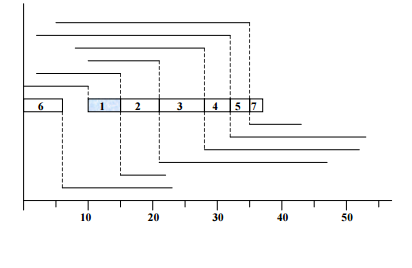
\includegraphics[scale=0.7]{wyk_1}
\caption{Wykres ustawienia elementów RPG na osi}
\end{figure}

\subsection{Podzial Zadania}
Zdefiniujmy zbiór $K = {c + 1, . . . , b}$. Zgodnie z definicją mamy $q_c < q_j , j \in K$. Łatwo zauważyć, że zachodzi $S_c < r_j$ , $j \in K$. Istotnie, gdyby zachodziło $S_c r_i$ dla pewnego $i \in K$, to zadanie $i$ byłoby gotowe do wykonywania w chwili czasowej $t = S_c$, w której podejmowano decyzje o uszeregowaniu zadania $c$, i zadanie to zostałoby uszeregowane w chwili $t$ zamiast $c$ ze względu na warunek $q_j > q_c$. Zatem otrzymujemy nierówność prawdziwą dla każdego $j \in K$.
 \begin{center}
 $r_j > S_c = r_a + \sum^{c+1}_{t=a}P_t$\\
 \end{center}
 implikującą oczywistą nierówność 
 \begin{center}
$r(K) = \underset{j \in K}{min} r_j > S_c = r_a +\sum^{c+1}_{t=a}P_t$. \\
\end{center}
Zgodnie z definicją zbioru $K$ mamy 
\begin{center}
$q_b = \underset{j \in K}{min} q_j = q(K)$.\\
\end{center}
Zatem ostatecznie
\begin{center}
 $h(K) = r(K) + p(K) + q(K) > r_a + p(I) + q_b - p_c = C_{max}(\pi) - p_c$\\
\end{center}
co kończy dowód własności. 

\begin{figure}[!ht]
\centering
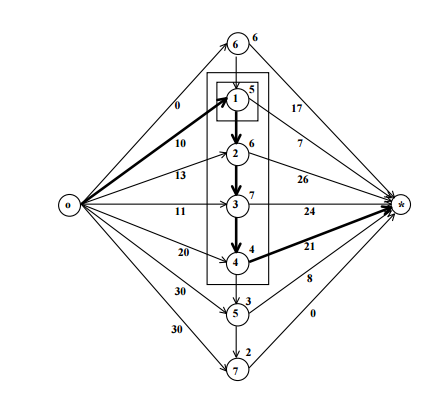
\includegraphics[scale=0.7]{wyk_2}
\caption{Interpretacja zadania c oraz zbioru K na grafie}
\end{figure}



Przyjmujemy początkowo $UB = \infty$. Wyznaczamy $\pi^S$ poprzez zastosowanie Algorytmu $S$, a w dalszej kolejności odpowiadającą mu wartość funkcji celu $C_{max}(\pi^S)$, drogę krytyczną $(a, b)$, zadanie interferencyjne $c$ oraz zbiór krytyczny $K$. Jeśli $c$ nie istnieje to otrzymane rozwiązanie jest optymalne dla rozważanego problemu. W przeciwnym przypadku kreowane są $2+1$ problemy potomne (następniki w drzewie rozwiązań), z których $2$ podlegają sprawdzeniu zaś jeden jest zawsze eliminowany. Dwa podstawowe problemy potomne są określone następująco:

\begin{itemize}
\item “zadanie $c$ jest wykonywane przed wszystkimi zadaniami ze zbioru $K$”. Warunek ten jest uwzględniany poprzez modyfikację danych problemu według zasady
\begin{center}
  $q_c := max{(q_c, p(K) + q_b)}$.
\end{center}
\item “zadanie $c$ jest wykonywane za wszystkimi zadaniami ze zbioru $K$”. Warunek ten jest uwzględniany poprzez modyfikację danych problemu według zasady
\begin{center}
   $r_c := max{(r_c, r(K) + p(K))}$
\end{center}
\end{itemize}

\subsection{Eliminacja}
Dla rozpatrywanej permutacji $\pi^S$ tworzony jest zbiór
 $L = {(i \in J / K : p_i > UB - h(K))}$.
 Jeśli $i \in L$ to $i$ musi być wykonywane przed lub za $K$. Odpowiednio budowane są dwa dodatkowe testy eliminacyjne 1. Jeśli $i \in L$ oraz
 \begin{center}
 $r_i + p_i + p(K) + q_b \ge UB)$
 \end{center}
 
to $i$musi być wykonywane za wszystkimi zadaniami z $K$ co pozwala na wykonanie modyfikacji
\begin{center}
$r_i := max({r_i , r(K) + p(K))} $
\end{center}

 Jeśli  $i \in L$ oraz
 \begin{center}
 $r(K) + p_i + p(K) + q_i\ge UB$
 \end{center}
 
 to i musi być wykonywane przed wszystkimi zadaniami z $K$ co pozwala na wykonanie modyfikacji 
 \begin{center}
 $q_i := max({q_i , q(K) + p(K))}$
 \end{center}


\section{ Wpływ strategii przeglądania i dodatkowych testów eliminacyjnych na efektywność pracy algorytmu:}
\subsection{Algorytm Carliera bez testów eliminacyjnych:
}
\begin{itemize}
\item Algorytm Carliera bez wyboru strategii:\\
\begin{table}[!ht]
  \begin{center}
    \begin{tabular}{| l | r |}
    \hline
   
data 0 &7 [ms]\\
data 1 & 374 [ms]\\
data 2 & 149853 [ms]\\
data 3 & 88 [ms]\\
data 4 & 18 [ms]\\
data 5 & 13569 [ms]\\
data 6 & 1076987 [ms]\\
data 7 & 38286357 [ms]\\
data 8 &>24h\\

    \hline
    \end{tabular}
  \end{center}
  \caption{Algorytm Carliera bez wyboru strategii}
\end{table}

\item  Algorytm Carliera z wyborem właściwej strategii przeglądania:\\
\begin{table}[ht!]
\centering
\label{my-label}
\begin{tabular}{|l|l|l|l|l|l|l|l|l|l|l|l|}
\hline
\multicolumn{12}{|c|}{z testami, bez strategii, czasy {[}ms{]}}           \\ \hline
       & 1  & 2  & 3  & 4   & 5  & 6  & 7  & 8  & 9  & 10 & średnia \\ \hline
data 0 & 30 & 3  & 2  & 4   & 2  & 1  & 1  & 28 & 1  & 1  & 7,3     \\ \hline
data 1 & 22 & 26 & 20 & 17  & 18 & 18 & 18 & 22 & 20 & 19 & 20      \\ \hline
data 2 & 35 & 35 & 38 & 33  & 27 & 31 & 28 & 38 & 29 & 28 & 32,2    \\ \hline
data 3 & 25 & 25 & 21 & 25  & 18 & 17 & 18 & 31 & 17 & 17 & 21,4    \\ \hline
data 4 & 34 & 34 & 35 & 33  & 26 & 30 & 27 & 35 & 26 & 31 & 31,1    \\ \hline
data 5 & 31 & 29 & 78 & 29  & 26 & 27 & 24 & 93 & 29 & 25 & 39,7    \\ \hline
data 6 & 74 & 80 & 70 & 100 & 65 & 65 & 68 & 68 & 63 & 93 & 74,6    \\ \hline
data 7 & 43 & 52 & 40 & 37  & 38 & 70 & 64 & 43 & 39 & 38 & 46,4    \\ \hline
data 4 & 22 & 17 & 18 & 14  & 23 & 30 & 23 & 21 & 22 & 27 & 21,7    \\ \hline
\end{tabular}
 \caption{Algorytm Carliera z wyborem właściwej strategii przeglądania}
\end{table}
\end{itemize}
\newpage
\subsection{Algorytm Carliera z testami eliminacyjnymi:}
\begin{itemize}
\item Algorytm Carliera bez wyboru strategii:\\
\begin{table}[!ht]
\centering
\label{my-label}
\begin{tabular}{|l|l|l|l|l|l|l|l|l|l|l|l|}
\hline
\multicolumn{12}{|c|}{bez testów, z wyborem strategii, czasy {[}ms{]}}           \\ \hline
       & 1  & 2   & 3   & 4   & 5   & 6  & 7   & 8  & 9   & 10  & średnia \\ \hline
data 0 & 2  & 2   & 1   & 2   & 1   & 1  & 1   & 3  & 4   & 139 & 15.6    \\ \hline
data 1 & 14 & 19  & 16  & 24  & 61  & 14 & 16  & 17 & 24  & 79  & 28.4    \\ \hline
data 2 & 26 & 43  & 47  & 47  & 56  & 35 & 36  & 38 & 39  & 76  & 44.3    \\ \hline
data 3 & 84 & 114 & 119 & 112 & 213 & 96 & 161 & 97 & 163 & 102 & 126.1   \\ \hline
data 4 & 10 & 23  & 21  & 28  & 31  & 20 & 15  & 16 & 19  & 17  & 20      \\ \hline
data 5 & 14 & 20  & 18  & 22  & 45  & 37 & 16  & 15 & 34  & 18  & 23.9    \\ \hline
data 6 & 22 & 24  & 25  & 69  & 25  & 19 & 19  & 20 & 28  & 20  & 27.1    \\ \hline
data 7 & 29 & 31  & 34  & 30  & 40  & 28 & 23  & 27 & 36  & 56  & 33.4    \\ \hline
data 8 & 64 & 26  & 27  & 30  & 26  & 28 & 21  & 21 & 28  & 26  & 29.7    \\ \hline
\end{tabular}
\caption{Algorytm Carliera z testami eliminacyjnymi}
\end{table}

\item Algorytm Carliera z wyborem właściwej strategii przeglądania:\\
\begin{table}[!ht]
\centering
\label{my-label}
\begin{tabular}{|l|l|l|l|l|l|l|l|l|l|l|l|}
\hline
\multicolumn{12}{|c|}{z testami, z wyborem strategii, czasy {[}ms{]}}       \\ \hline
       & 1   & 2  & 3  & 4  & 5  & 6  & 7  & 8   & 9  & 10  & średnia \\ \hline
data 0 & 34  & 10 & 31 & 9  & 2  & 2  & 4  & 3   & 2  & 1   & 9.8     \\ \hline
data 1 & 17  & 30 & 20 & 33 & 19 & 17 & 19 & 19  & 21 & 24  & 21.9    \\ \hline
data 2 & 39  & 28 & 32 & 41 & 38 & 34 & 31 & 30  & 36 & 49  & 35.8    \\ \hline
data 3 & 35  & 88 & 24 & 27 & 54 & 23 & 51 & 175 & 31 & 32  & 54      \\ \hline
data 4 & 42  & 38 & 27 & 27 & 39 & 24 & 31 & 27  & 31 & 45  & 33.1    \\ \hline
data 5 & 23  & 36 & 24 & 30 & 20 & 24 & 31 & 111 & 56 & 35  & 39      \\ \hline
data 6 & 109 & 86 & 39 & 40 & 44 & 44 & 53 & 49  & 35 & 59  & 55.8    \\ \hline
data 7 & 29  & 35 & 35 & 33 & 33 & 33 & 46 & 41  & 26 & 139 & 45      \\ \hline
data 8 & 13  & 69 & 53 & 20 & 21 & 25 & 23 & 19  & 23 & 24  & 29      \\ \hline
\end{tabular}
\caption {Algorytm Carliera z wyborem właściwej strategii przeglądania}
\end{table}
\end{itemize}


\section{Porównanie trzech wariantów algorytmu Carliera:} 
\begin{itemize}
\item bez testów eliminacyjnych, z wyborem właściwej strategii przeglądania
\item z testami eliminacyjnymi, z wyborem właściwej strategii przeglądania
\item z testami eliminacyjnymi, bez wyboru strategii

\end{itemize}

\begin{figure}[!h]
\centering
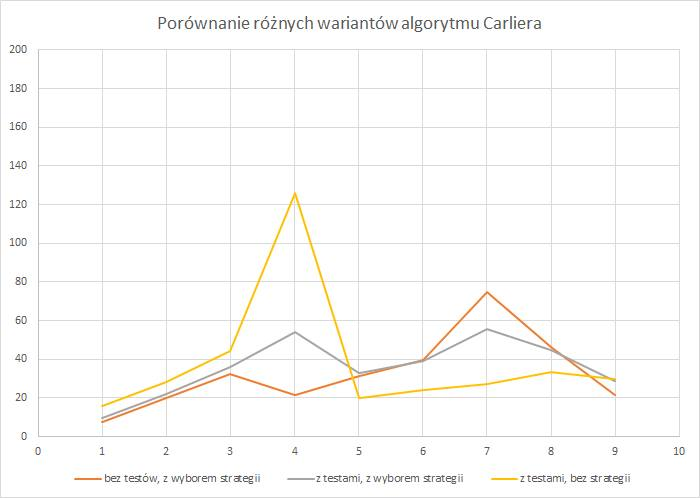
\includegraphics[scale=0.6]{Wykres_1}
\caption{Interpretacja zadania c oraz zbioru K na grafie}
\end{figure}

 Algorytm Carliera bez wyboru właściwej strategii oraz bez testów eliminacyjnych:

\begin{figure}[!h]
\centering
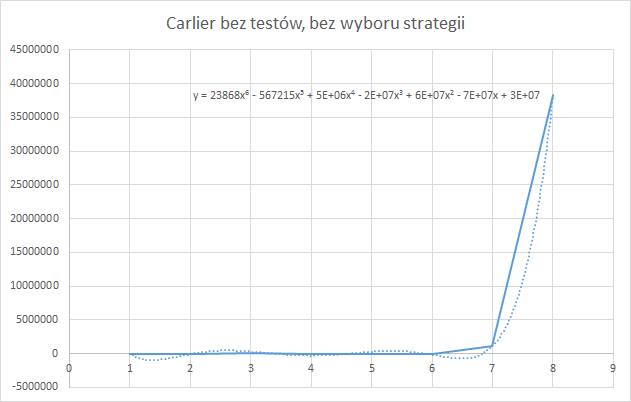
\includegraphics[scale=0.6]{wykres_2}
\caption{Interpretacja zadania c oraz zbioru K na grafie}
\end{figure}

\newpage
\section{Wnioski} 
~~~~Jak widać algorytm jest bardzo czasochłonny, przeprowadzenie eksperymentu zajęło ponad trzy dni, już na siódmym zestawie danych algorytm wykonywał się w 10 godzin, a długość obliczeń na zestawie ósmym to już ponad 24 godziny. Dla sprawdzenia jaki czasochłonny jest algorytm, w excelu dodano linię trendu, złożoność algorytmu wynosi $O(x^6)$.

Uzupełnienie badał z użyciem Schrage i Schrage z podzialem o dodatkowe testy eliminacyjne
oraz odpowiednią strategię przeglądania przyspieszyło przeglądanie węzłów przez szybszą ich eliminację i przeglądanie najbardziej prawdopodobnych gałęzi

Zastosowanie dodatkowych testów eliminacyjnych oraz wybór właściwej strategii przeglądania pozwoliło znacząco skrócić czas obliczania, złożoność algorytmu wynosi O(1), ponieważ utrzymuje się mniej więcej na tym samym poziomie poziomie, występują małe, prawie niezauważalne zmiany.

Można zauważyć, że wśród danych wejściowych otrzymujemy zestawy lepiej i gorzej ułożone. Bardzo dużo problemów pojawiło się przy zestawie data.8 oraz data.7, głównie  przy wykonywaniu algorytmu Carliera bez dodatkowych testów eliminacyjnych oraz bez wyboru strategii.

W przypadku małych ilości danych algorytm Carliera nie ma problemu nawet bez wyboru strategii, co można zauważyć w przypadku dane.0, gdy liczba danych=4. Także nie występują problemy z obliczeniem jeżeli dane są korzystnie ułożone, na podstawie eksperymentów możemy stwierdzić, że takim zestawem dobrze ułożonym jest zestaw data.4.

W czasie wykonywania eksperymentu bez testów eliminacyjnych oraz bez wyboru strategii procesor wykorzystywał 70\% swojej mocy do obliczeń, mimo to, program wykonywał się  ponad trzy dni, co znacząco utrudniło testy, należało je zacząć odpowiednio wcześniej.

Do algorytmu zostało także dodane odkładanie podproblemów na kopcach. Każdy z elementów kopca otrzymuje oznaczenie po której stronie się znajduje (lewa, prawa).

Uzupełnienie badał z użyciem Schrage i Schrage z podzialem o dodatkowe testy eliminacyjne
oraz odpowiednią strategię przeglądania przyspieszyło przeglądanie węzłów przez szybszą ich eliminację i przeglądanie najbardziej prawdopodobnych gałęzi.


\begin{thebibliography}{9}
\bibitem{Makuchowski} 
M Makuchowski,
\textit{dostęp z dnia 30.05.2016 r.1}. \\
http://mariusz.makuchowski.staff.iiar.pwr.wroc.pl/download/courses/sterowanie.procesami.dyskretnymi/\\lab.instrukcje/lab05.carlier/carl.literatura/%5bAS%5d.carlier.pdf

\bibitem{Makuchowski}
M. Makuchowski,
\textit{dostęp z dnia 30.05.2016 r.1}
mariusz.makuchowski.staff.iiar.pwr.wroc.pl/
downloadcoursessterowanie.procesami.dyskretnymi
/lab.instrukcjelab04.schrageschr.literaturaa.schrage.pdf
 
\bibitem{Smutnicki} 
Cz. Smutnicki,\\
\textit{Algorytmy szeregowania zadań, Oficyna Wydawnicza Politechniki Wrocławskiej, Wrocław 2012}. 
 
\end{thebibliography}


\end{document}
